\scanpage{43}
\margin{?}
\uline{NB} Si $X_0$ est un schéma abélien \deleted{\unsure{plat|alors}} (ou seulement para-abélien), alors ces conditions \deleted{impliquent} \inserted{équivalent à celle (0)} que $\mathfrak X$ soit algébrique, et dans l'énoncé des conditions (i) à (iv) [dont d'ailleurs seules (i) et (ii) sont \unsure{intrinsèques|intéressantes}] on peut supprimer la condition de projectivité.

\uline{Remarque.} Soit $S'\mathbin{-}S$ un
\inserted{\figure{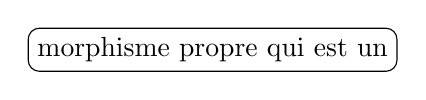
\begin{tikzpicture}\node[draw,rounded corners] {morphisme propre qui est un};\end{tikzpicture}}}
(épimorphisme) effectif (de loc noeth). C'est donc un morphisme de descente effective pour les schémas relatifs plats. Soit $X'$ plat et propre sur $S'$, avec donnée de descente à $S$, on \deleted{\unsure{veut}} se demande si donnée de descente est effective.

\deleted{a) Condition locale sur $S$}
a) On peut se réduire aux localisés \inserted{$\mathcal O_{S,s}$} de $S$.

b) Moyennant une question de descente \deleted{\unsure{fid}} \inserted{fid.} plate, on est ramené au pb sur $\widehat{\mathcal O}_{S,s}$. Il peut être intéressant d'avoir \deleted{\unsure{de plus}} assez de $\unsure{V^{\mathrm t}}$ de $X_s$, et pour ceci de faire comme une cat. \unsure{fibrée} \deleted{\unsure{étale}} \inserted{\unsure{étale} $\unsure{R}$} de $\widehat{\mathcal O}_{S,s}$. On peut alors supposer que $X_s$ sur le corps résiduel $k$ de $R$, on peut descendre, donc \unsure{isom.} à un $X_0$.

\margin{\uline{\unsure{Conditions} \unsure{sans} \unsure{doute} \unsure{inutiles}}}
c) Supposons \inserted{la réduction précédente faite, et} que les fibres de $X'/S'$ soient sans aut. infinitésimaux, et que $X'$ \deleted{soit lisse sur $S'$} ait \deleted{\unsure{une}} ``assez'' de sections \deleted{\unsure{dont} \unsure{le long}} \deleted{\unsure{desquelles}} plates par descente, le long desquelles $X'/S'$ soit lisse. Alors un argument de modules formels permet de construire un schéma formel $\widehat X$ sur $\widehat S$ qui descend $\widehat X'$.

\mspage{42}
